\newpage
%\pagestyle{empty}

\begin{minipage}[c]{.25\linewidth}
	
\includegraphics[width=4cm]{images/LEnsE_IOGS.jpg}
\end{minipage} \hfill
\begin{minipage}[c]{.4\linewidth}

\begin{center}
\vspace{0.3cm}
{\Large \textsc{Opto-Électronique}}

\medskip

5N-027-SCI \qquad \textbf{\Large TD Séance 2}

\end{center}
\end{minipage}\hfill

%%%%%%%%%%%%%%%%%%%%%%%%%%%%%%%%%%
\section{TD2 - Amplificateur Linéaire Intégré (ALI)}

Aussi appelé \textbf{Amplificateur Opérationnel} (AOP)

%%%%%%%%%%%%%%%%%%%%%%%%%%%%%%%%%%%%%%%%%%%%%%%%%%%%%%%
\subsection{Exercice 1 - Amplificateur linéaire intégré}
On fournit en annexe une partie de la documentation technique de l'amplificateur linéaire intégré (ALI) \textbf{TL081}.

\begin{enumerate}
	\item Cherchez dans la documentation les valeurs des paramètres électriques suivants :
	\begin{enumerate}
		\item Tension d'alimentation (Supply Voltage)
		\item Tension d'entrée différentielle maximale
		\item Amplification différentielle 
		\item Gain unitaire ou produit gain-bande-passante
		\item Impédance d'entrée 
		\item Slew Rate
	\end{enumerate}
	\item Précisez à quoi corresponde chacun de ces paramètres.
	\item Rappelez la relation entre les entrées $V^+$, $V^-$ et la sortie $V_S$ d'un ALI.
	\item Tracez la caractéristique $V_S = f (\varepsilon)$ où $\varepsilon = (V^+ - V^-)$ pour cet ALI avec $V_{CC} = 15\operatorname{V}$.
	\item Est-ce un bon amplificateur ? Quelle est sa bande-passante ?

\end{enumerate}

\subsection*{Réponse}

%%%%%%%%%%%%%%%%%%%
\textbf{Question 1}

\begin{itemize}
	\item Tension d'alimentation (Supply Voltage) = 18V
	\item Tension d'entrée différentielle maximale = 30V
	\item Amplification différentielle - $A_{VD} = 200\operatorname{V/mV} = 2 \cdot 10^5$
	\item Gain unitaire ou produit gain-bande-passante - $B_1 = 3\operatorname{MHz}$ 
	\item Impédance d'entrée - $r_i = 10^{12}\operatorname{\Omega} = 10^6\operatorname{M\Omega} = 1\operatorname{T\Omega}$
	\item Slew Rate - $SR = 13\operatorname{V/\mu{}s}$
\end{itemize}

\textbf{Question 2}

\begin{itemize}
	\item Tension d'alimentation : les ALI sont des composants actifs, ils nécessitent une source d'énergie pour fonctionner. Ici il est nécessaire de réaliser une source de tension symétrique, c'est à dire une source positive $+V_{CC}$ et une source négative $-V_{CC}$, où $V_{CC} < 18\operatorname{V}$
	\item Tension d'entrée différentielle maximale : c'est la différence de potentiel maximale admissible entre $V^+$ et $V^-$. On appelle tension d'entrée différentielle $\varepsilon = (V^+ - V^-)$
	\item Amplification différentielle : c'est l'amplification du composant, le lien entre la tension de sortie ($V_S$) et la tension différentielle d'entrée ($\varepsilon$).
	\item Gain unitaire ou produit gain-bande-passante : c'est une donnée essentielle qui permet de connaître la bande-passante du composant lorsque l'amplification du montage est de 1. Sur les montages amplificateurs (à base d'ALI), le produit amplification bande-passante est constant. 
	\item Impédance d'entrée : c'est l'impédance vu par le montage en amont de l'ALI.
	\item Slew Rate : cette donnée caractérise la pente maximale que pourra avoir l'ALI en sortie.
\end{itemize}

\textbf{Question 3}

$$V_S = A_{VD} \cdot (V^+ - V^-)$$

avec $A_{VD} = 200\operatorname{V/mV} = 2 \cdot 10^5$ (dans le cas du TL081).

\textbf{Question 4}

Courbe avec saturation à +/-15V (dans le cas d'une alimentation où $V_{CC} = 15\operatorname{V}$. 

La saturation en sortie apparait pour une valeur de $\varepsilon = V_{CC} / A_{VD}$. Pour $V_{CC} = 15\operatorname{V}$, on a $\varepsilon_{MAX} = V_{CC} / A_{VD} = 75\operatorname{\mu{}V}$.

\textbf{Question 5}

L'amplication différentielle est souvent supérieure à $10^5$, c'est donc un très bon amplificateur.

Cependant, il a un produit amplification/bande-passante ($GBW$) qui est constant et "faible", ce qui le rend finalement peu efficace pour des fréquences élevées en boucle ouverte.

Par exemple, pour un $GBW = 3\operatorname{MHz}$ et une amplification différentielle $A_{VD} = 2 \cdot 10^5$ (cas du TL081), on obtient une bande-passante en boucle ouverte (sans rebouclage) $f_c = GBW / A_{VD} = 15\operatorname{Hz}$.

\newpage
%%%%%%%%%%%%%%%%%%%%%%%%%%%%%%%%%%%%%%%%%%%%%%%%%%%%%%%
\subsection{Exercice 2 - Montage amplificateur inverseur}
On se propose d'étudier à présent le montage suivant :

\begin{center}
\begin{circuitikz} 
	\node [op amp, fill=blue!10!white](A1) at (0,0){\texttt{AOP1}};
	\draw (A1.-) to[short] ++(-.5,0) coordinate(A) to[short] ++(0,1.5) coordinate(B) to[R=$R_2$] (B -| A1.out) to[short, -*] (A1.out);
	\draw (A1.-) to[short,-*] ++(-.5,0) coordinate(AA) to[R=$R_1$] ++(-2.5,0) coordinate(BB) to[short,-o] ++(-.5,0) coordinate(CC);
	\draw (A1.+) to[short] ++(0,-0.5) node[ground]{};
	\draw (A1.out) to[short,-o] ++(1,0) coordinate(D);
	\draw (-4.6,-1) edge[->,color={green!40!black}] (-4.6,0.3);
	\node[text={green!40!black}] (Ve) at (-5.1,-0.35){$V_e$}; 
	\draw (-4.6,-1.3)  to[open,-o] ++(0,0) node[ground](GND){};
	\draw (2.2,-1) edge[->, color={red}] (2.2,-0.3);
	\node[text={red}] (Vs) at (1.7,-0.6){$V_s$}; 
	\draw (2.2,-1.3)  to[open,-o] ++(0,0) node[ground](GND){};
	
\end{circuitikz}
\end{center}

\begin{enumerate}
	\item Donnez la relation entre $V_S$ et $V_E$ du circuit précédent en utilisant la relation d'entrées-sortie de l'exercice 1.
	\item Quelle hypothèse fait-on souvent lorsqu'on utilise des ALI avec une rétroaction négative ?
	\item Quelle relation trouve-t-on alors entre $V_S$ et $V_E$ en partant de cette hypothèse ?
	\item Cette hypothèse est-elle justifiée ?
\end{enumerate}


\subsection*{Réponse}

%%%%%%%%%%%%%%%%%%%
\textbf{Question 1}

On calcule d'abord les potentiels $V^+$ et $V^-$ en entrée de l'ALI (théorème de Millman) :

$$V^- = \frac{\frac{V_S}{R_2} + \frac{V_E}{R_1}}{\frac{1}{R_2} + \frac{1}{R_1}} = \frac{V_S \cdot R_1}{R_1 + R_2} + \frac{V_E \cdot R_2}{R_1 + R_2}$$

$$V^+ = 0$$

De plus, on sait que $V_S = A_{VD} \cdot (V^+ - V^-)$

On obtient alors : $$V_S = - A_{VD} \cdot \frac{\frac{V_S}{R_2} + \frac{V_E}{R_1}}{\frac{1}{R_2} + \frac{1}{R_1}} = \frac{V_S \cdot R_1}{R_1 + R_2} + \frac{V_E \cdot R_2}{R_1 + R_2}$$

Ce qui donne : $$T = \frac{V_S}{V_E} = - \frac{R_2}{R_1} \cdot \frac{A}{A + \frac{R_1 + R_2}{R_1}}$$


\textbf{Question 2}

$V^+ = V^-$

Lorsqu'on reboucle la sortie sur l'entrée négative sur un ALI, on change son régime de fonctionnement. Il s'agit d'un système bouclé (ou asservi). La sortie va chercher à suivre un signal de consigne appliqué sur l'entrée positive et ainsi l'erreur commise ($V^+ - V^-$) va tendre vers 0.


\textbf{Question 3}

Les relations obtenues dans la question 1 pour $V^+$ et $V^-$ restent vraies. Ainsi : 
$$V^- = \frac{\frac{V_S}{R_2} + \frac{V_E}{R_1}}{\frac{1}{R_2} + \frac{1}{R_1}} = \frac{V_S \cdot R_1}{R_1 + R_2} + \frac{V_E \cdot R_2}{R_1 + R_2}$$

$$V^+ = 0$$

De plus, en faisant l'hypothèse $V^+ = V^-$, on obtient : $$T = \frac{V_S}{V_E} = - \frac{R_2}{R_1}$$

\textbf{Question 4}

On passe de l'expression obtenue à la question 1 à celle de la question 3 lorsqu'on suppose que $A_{VD} >> \frac{R_1 + R_2}{R_1}$.

Il est fréquent de prendre des valeurs de résistances telles que $R_2 / R_1 \approx 10$. Cette hypothèse est avérée dans le majorité des cas.


\textbf{Exemple}

On souhaite montrer ici l'erreur commise sur la valeur de l'amplification entre la formule complète (incluant l'amplification différentielle) et l'approximation faite en régime linéaire, en fonction de l'amplification $R_2 / R_1$ voulue pour le système.

Pour cela, on fixe $A_{VD} = 15 \cdot 10^3$ la valeur minimale que l'on trouve dans la documentation technique du TL081 (par exemple) et on fait varier le rapport $R_2 / R_1$ de $2$ à $10^3$.


On obtient alors la figure suivante : 

\begin{center}
	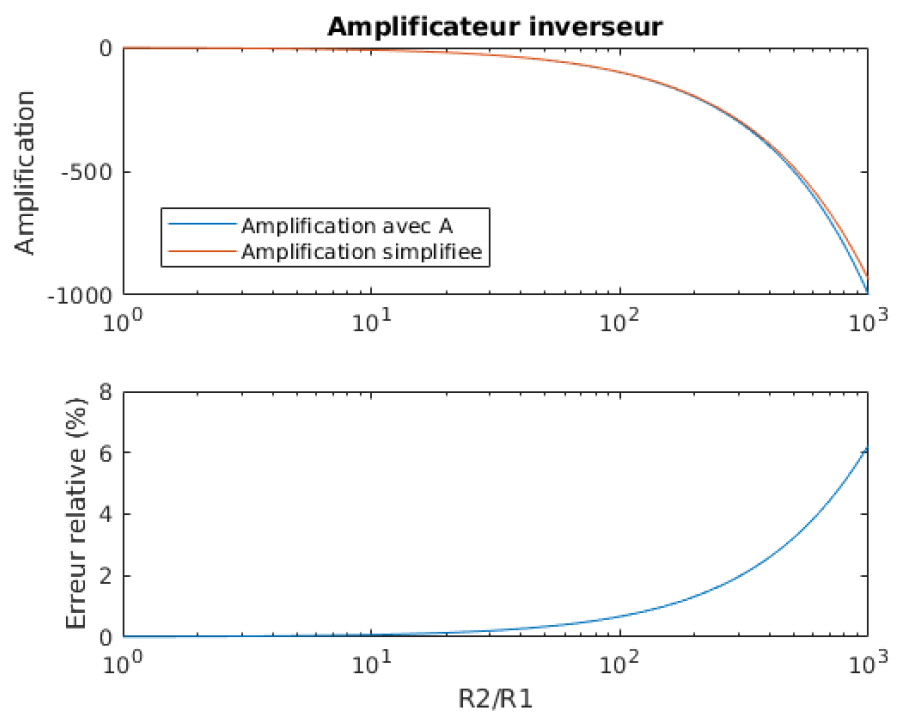
\includegraphics[width=11cm]{images/ampliinv_002_cor_a.png}
\end{center}

\newpage
%%%%%%%%%%%%%%%%%%%%%%%%%%%%%%%%%%%%%%%%%%%%%%%%%%%%%%%
\subsection{Exercice 3 - Mettre en forme un capteur de température}
On se propose d'étudier le circuit suivant :

\begin{center}
	
\includegraphics[width=16cm]{images/capteur_conditionnement.png}
\end{center}

La thermistance utilisée est de type PT100. La relation entre sa résistance (en Ohms) et la température (en \degre{}C) est la suivante :
$$R(T) = 100~(1 + 3.908×10^{-3} T - 5.802×10^{-7} T^2)$$


\begin{enumerate}
	\item Découpez le montage précédent en sous-ensemble.
	\item Donnez la relation de $V_S$ en fonction de $R(T)$ et de $V_Z$. 
\end{enumerate}


\subsection*{Réponse}

%%%%%%%%%%%%%%%%%%%

\textbf{Etude du montage}

Pour étudier ce circuit, on commence par \textbf{décomposer en blocs} plus facilement calculables, en partant du signal de sortie.

De manière générale, chaque amplificateur linéaire (ALI) correspond à un montage particulier. Il peut donc être intéressant d'identifier les montages associés à chaque ALI.

Ici, on peut décomposer de cette façon : 
\begin{itemize}
	\item Autour de l'AO4 : amplificateur différentiel 
	\item Autour des AO2 et AO3 : suiveur / découplage
	\item Autour de l'AO1 : montage linéaire de type amplificateur / tension de sortie dépendante de la température
	\item Autour de la diode Zener : tension de référence	
\end{itemize}


\textbf{AO1} 

Hypothèse classique : fonctionnement linéaire ($V^+ = V^-$) et ALI parfait ($i^+ = i^- = 0$).

$V+ = V_Z \cdot R_2 / (R_1 + 2 R_2)$ et $V- = V_1 \cdot R_2 / (R_2 + R(T))$, alors : 

$$V_1 = V_Z \cdot \frac{R_2}{R_1 + 2 R_2} \cdot \frac{R_2 + R(T)}{R_2} = V_Z \cdot \frac{R_2 + R(T)}{R_1 + 2 R_2}$$

\textbf{AO2} : suiveur / diviseur de tension

$$V_2 =  V_Z \cdot \frac{2 \cdot R_2}{R_1 + 2 R_2}$$

\textbf{AO3} : suiveur

$$V_3 = V_1$$

\textbf{AO4} 

$V- = (V_S/R_4 + V_2/R_3) / (1/R_3 + 1/R_4)$ (Millmann)

$V+ = V_3 \cdot R_4 / (R_3 + R_4)$

On a alors : 

$$V_S = (V_3 - V_2) \cdot \frac{R_4}{R_3}$$


\textbf{Montage complet}

$$V_S = V_Z \cdot \frac{R_4}{R_3} \cdot \frac{R(T) - R_2}{R_1 + 2 R_2}$$

$$V_S = V_Z \cdot \frac{R_4}{R_3} \cdot \frac{R_2}{R_1 + 2 R_2} \cdot (\frac{R(T)}{R_2} - 1)$$


Lorsque $T < 0$, $R(T) < R_2$ et donc $V_S < 0$. Alimentation symétrique indispensable.

%%%%%%%%%%%%%%%%%%%%%%%%%%%%%%%%%%%%%%%%%%%%%%%%%%%%%%%

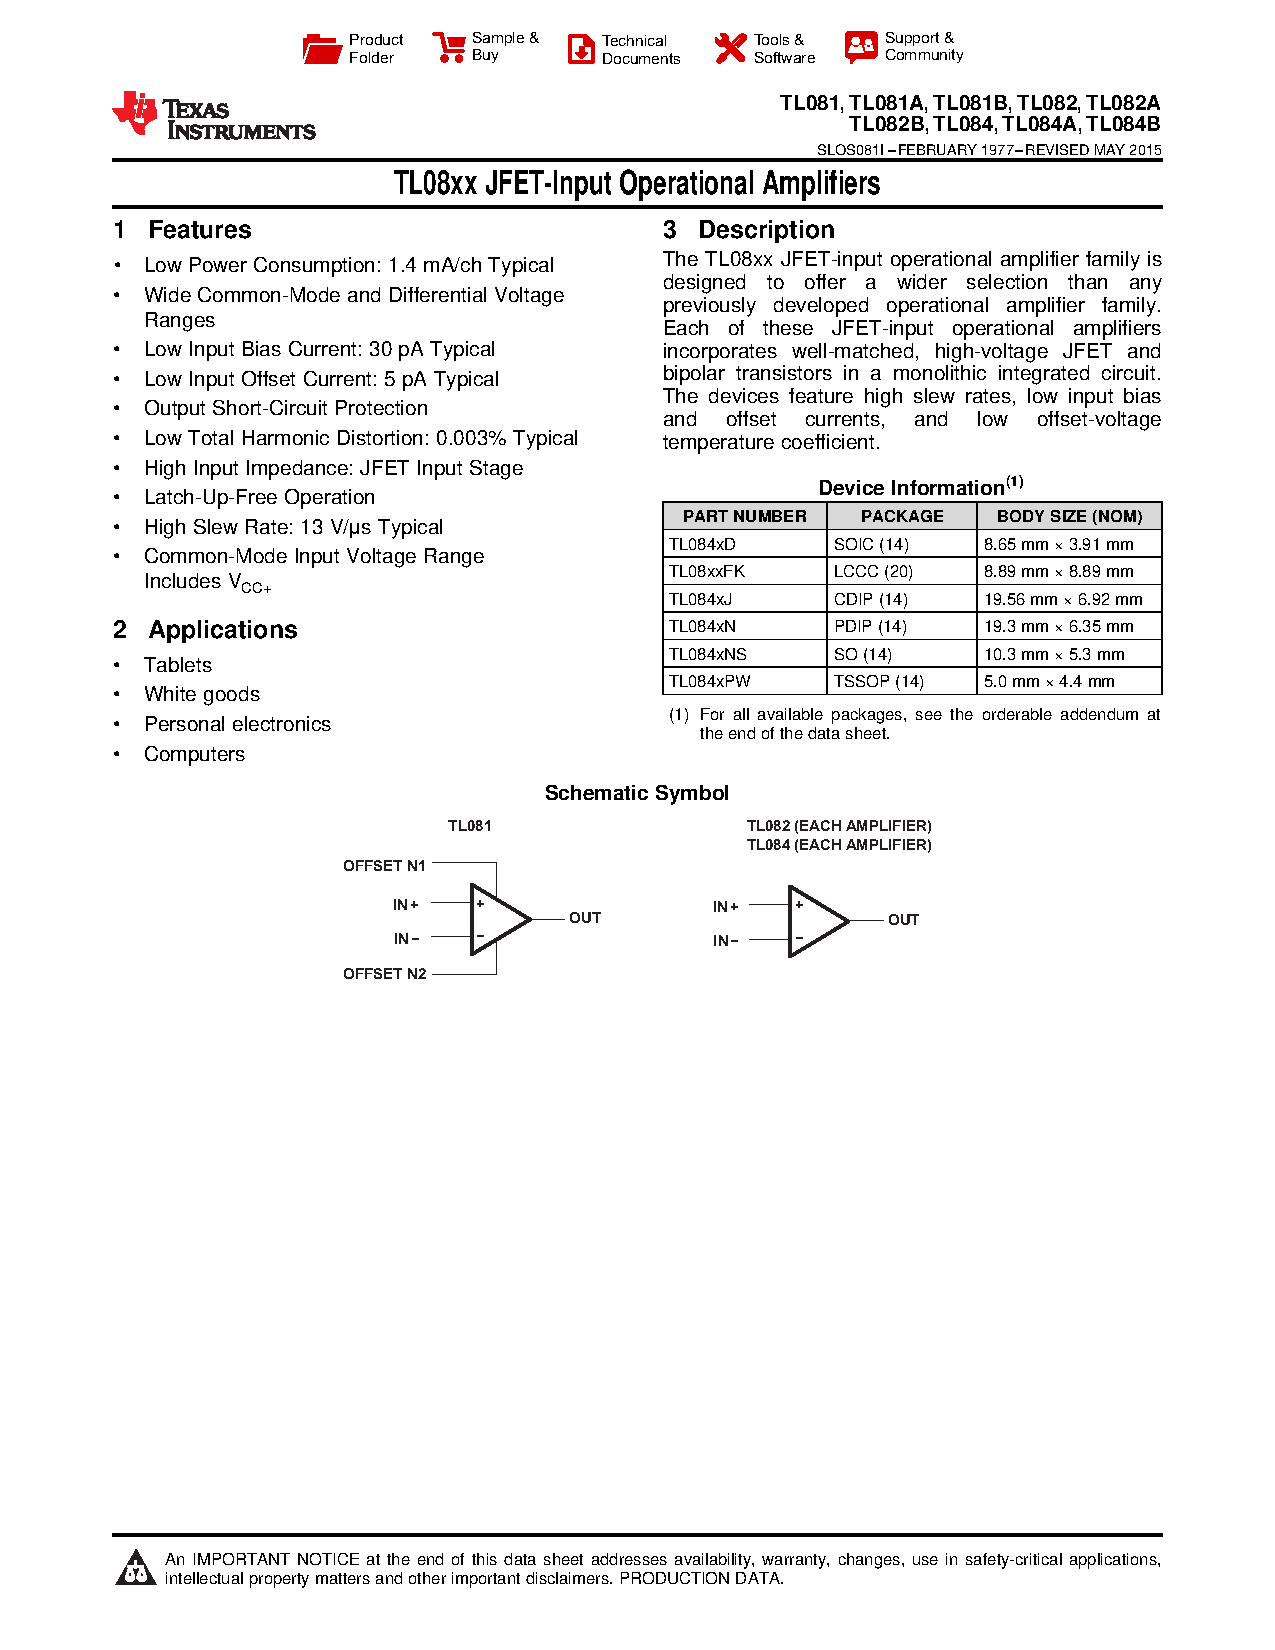
\includepdf[pages=-]{docs/doc_TL071_1p.pdf}

%%%%%%%%%%%%%%%%%%%%%%%%%%%%%%%%%%%%%%%%%%%%%%%%%%%%%%%